\chapter{Подход к поиску путей в графе с  КС-ограничениями на основе методов линейной алгебры}\label{ch:ch2}

В этой главе представлен подход к решению класса задач по поиску путей в графе с ограничениями, заданными КС-языком, с помощью методов линейной алгебры. То есть на вход предлагаемый подход получает описание задачи указанного класса, а на выходе выдает алгоритм и некоторые другие артефакты. Несмотря на то, что полностью детерминированную процедуру для создания таких алгоритмов создать не удаётся, видится целесообразным аккумулировать успешный опыт создания ряда алгоритмов этого класса в виде предлагаемого ниже подхода. Этот подход может быть использован как руководство, он также содержит успешные примеры и отсылки к необходимым теоретическим результатам и программным библиотекам. Но он не заменяет акт творческого включения и удачи~--- это создателям алгоритмов для решения задач из указанного класса придётся обеспечить самостоятельно.    

В начале главы предлагается детальное описание предлагаемого подхода. После этого демонстрируется его использование для частного случая задачи поиска путей в графе с заданными КС-ограничениями, в котором ограничения задаются регулярными языками. В конце проведён анализ применимости и ограничений предложенного подхода.

\section{Описание подхода}
%Описание подхода (детальное описание каждого кубика)
Обобщая опыт Лэсли Вэлианта создания матричного алгоритма синтаксического анализа строк, а также подхода \textit{Algebraic Path Problem}, в данном диссертационном исследовании предлагается подход для решения задач поиска путей в графе с КС-ограничениями с помощью методов линейной алгебры.

Схема предлагаемого подхода изображена на~\cref{fig:schema}. В качестве фундамента выступают знания из следующих областей: линейная алгебра, теория формальных языков и теория графов. Аппарат линейной алгебры предоставляет: алгоритмы вычисления операций над матрицами и векторами, с помощью которых будет производиться анализ графов; методы решения систем линейных уравнений (такие системы могут возникнуть в матричной форме в процессе построения алгоритма анализа графа); теоретические свойства таких алгоритмов и методов, которые будут во многом определять теоретические свойства результирующего алгоритма; практические результаты в виде готовых высокопроизводительных библиотек линейной алгебры, которые будут использованы в реализации построенного алгоритма. Из теории графов используются: способы представления информации о графах и их связь с объектами линейной алгебры; существующие алгоритмы обхода и поиска путей в графе, которые послужат основой для алгоритмов поиска путей в графе с заданными КС-ограничениями; успешный опыт решения задач анализа графов с помощью методов линейной алгебры, который хорошо описан в книге~\cite{kepner2011graph}, а для задач поиска путей в графе собран в виде подхода \textit{Algebraic Path Problem}~\cite{rote1990path,baras2010path,chen1992parallel,lengauer1991unstructured}; практический опыт применения методов линейной алгебры к задачам анализа графов, который представлен в виде стандарта GraphBLAS~\cite{graphblas} и его реализаций. В свою очередь, теория формальных языков предлагает: способы описания КС-языков (формальные грамматики, рекурсивные автоматы), которые будут применены в построенном алгоритме для описания КС-ограничений на пути в графе; нормальные формы КС-грамматик и алгоритмы преобразования грамматик в эти нормальные формы, которые позволят использовать более простые правила вывода для описания ограничений на пути в графе.

На вход предлагаемый подход получает некоторую задачу поиска путей в графе с заданными КС-ограничениями. Такие задачи имеют множество формулировок и могут  различаться по следующим измерениям:
\begin{itemize}
    \item по виду искомой информации о путях в графе (задача достижимости, поиска одного пути, поиска всех путей);
    \item по множеству пар вершин графа, являющихся концами искомых путей (поиск путей между всеми парами вершин, фиксированное множество начальных вершин, одна начальная и одна конечная вершины и т.д.);
    \item по наличию дополнительных ограничений на искомые пути в графе в зависимости от решаемой задачи~--- поиск кратчайших путей, простых путей и т.д.
\end{itemize}

\begin{figure}
    \centering
	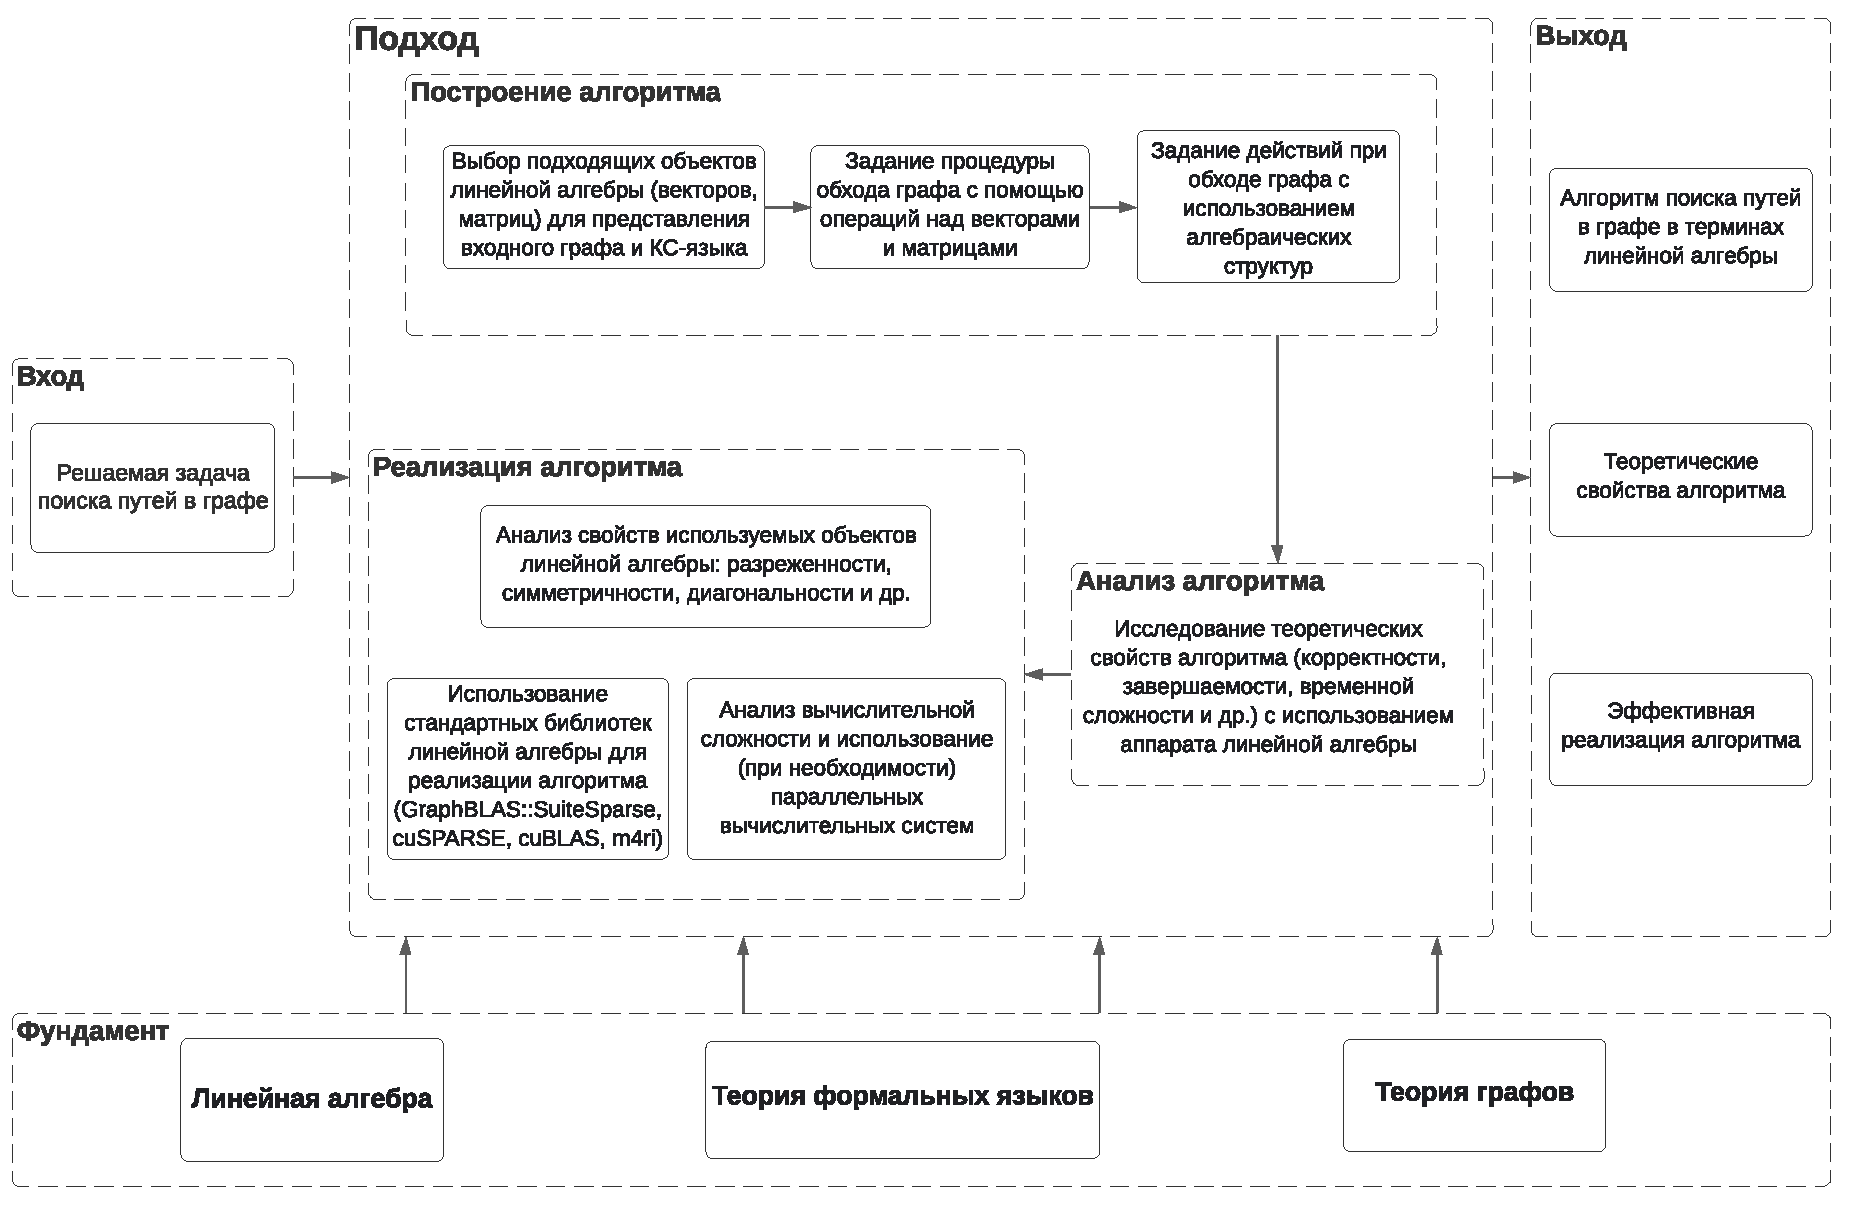
\includegraphics[width = 17.8cm]{Dissertation/images/schema.pdf}
	\caption{Схема подхода к поиску путей в графе с заданными КС-ограничениями с использованием методов линейной алгебры}
	\label{fig:schema}
\end{figure}

Стоит отметить, что решаемая задача может иметь практическую или теоретическую направленность. Например, при практической направленности целью применения предлагаемого подхода может быть получение высокопроизводительной реализации для решения поставленной задачи анализа графов. А при теоретической направленности основным результатом может являться получение алгоритма, который обладает некоторыми уникальными теоретическими свойствами.

Также при постановке решаемой задачи может указываться некоторая дополнительная информация про анализируемые графы и используемые КС-ограничения. Например, может быть известна степень разреженности графов или их особый вид (например, что на вход алгоритму будут подаваться только ацикличные графы). Это, в свою очередь, позволит использовать те или иные специфические структуры для хранения информации о графах, а также операции над этими структурами. Для хранения матриц смежности разреженных графов следует выбирать соответствующие разреженные форматы CSR, CSC, COO. А в случае ацикличности графов~--- их матрицы смежности будут иметь треугольный вид, что уменьшит сложность вычисления некоторых операций над ними. Например, первый этап метода Гаусса для решения системы линейных уравнений может быть пропущен, так как он приводит матрицу к треугольной форме. А такая операция, как вычисление транзитивного замыкания для треугольной матрицы имеет сложность, равную сложности вычисления одного умножения матриц. Аналогично, могут быть учтены особенности КС-языков, используемых в качестве КС-ограничений, для поиска наиболее подходящей структуры хранения этих ограничений и операций над этой структурой. Так, если перевод формальной грамматики для заданного КС-языка приводит к слишком значительному увеличению размеров этой грамматики, то целесообразно вместо такой трансформации использовать представление КС-языка в виде рекурсивного автомата. Кроме того, если заданные КС-ограничения соответствуют некоторому подклассу класса КС-языков (например, регулярным языкам), то целесообразно использовать соответствующие более простые структуры (например, конечные автоматы) для описания таких ограничений.

Предлагаемый подход делится на следующие части:
\begin{itemize}
    \item построение алгоритма поиска путей в графе с заданными КС-ограничениями в терминах линейной алгебры;
    \item анализ теоретических свойств построенного алгоритма и поставленной задачи;
    \item реализация построенного алгоритма.
\end{itemize}

Важной частью предлагаемого подхода является само построение алгоритма. Как и при решении других задач анализа графов, ключевым здесь является выбор подходящих объектов линейной алгебры (векторов, матриц) для представления информации о графах. Также подобные объекты можно использовать для представления КС-ограничений путём сведения КС-языков к рекурсивным автоматам~\cite{alur2005analysis} с последующим представлением этих автоматов в виде графов. Для представления информации о графах в подавляющем большинстве алгебраических алгоритмов анализа графов используются матрицы смежности (алгоритм обхода в ширину, алгоритм Беллмана-Форда, алгоритм Флойда-Уоршалла)~\cite{kepner2011graph}. Однако в некоторых из них также используются вектора (в алгоритме Беллмана-Форда для хранения расстояний от стартовой вершины до всех остальных; в алгоритме обхода в ширину один вектор~--- для хранения набора вершин, обрабатываемых на текущей итерации, другой~--- для хранения информации о всех вершинах графа, достижимых из стартовой). Таким образом, для представления графов следует использовать матрицы смежности, а для хранения информации о вершинах графа (достижимость из стартовой вершины; расстояние от стартовой вершины; набор вершин, инцидентных заданной вершине) следует использовать вектора.


Далее необходимо задать процедуру обхода графа. Как уже указывалось выше, при удачном выборе объектов линейной алгебры на предыдущем шаге  эта процедура может быть осуществлёна с помощью  операций над выбранными объектами~--- операциями над матрицами и векторами. Так, например, в алгоритме поиска транзитивного замыкания~\cite{baras2010path} для обхода графа используется ряд умножений матриц, а именно, возведений матриц во вторую степень. А в алгоритме Беллмана-Форда~\cite{kepner2011graph} на каждой итерации рассматриваются пути определённой длины с помощью умножения вектора на матрицу смежности. Следует отметить, что в алгоритмах поиска путей между всеми парами вершин используется умножение матрицы на матрицу, а в случае фиксированной стартовой вершины обход графа осуществляется с использованием умножения вектора на матрицу.


Далее, при успешном выполнении предыдущего шага, необходимо задать дополнительные действия в процессе обхода графа, позволяющие анализировать рассматриваемые пути и проверять их на соответствие заданным КС-ограничениям. Здесь предлагается рассмотреть алгебраические структуры, над которыми будут существовать введенные выше объекты линейной алгебры.  

Эти действия могут быть выполнены путём модификации выбранных операций над матрицами и векторами с использованием различных алгебраических структур (полуколец, моноидов и т.д.). Такие модификации с помощью полуколец широко используются для решения задач поиска путей и являются основной идеей подхода \textit{Algebraic Path Problem}~\cite{rote1990path}. Например, в алгоритме Беллмана-Форда для модификации операции умножения вектора на матрицу используется полукольцо $\langle \mathbb{R} \cup \{\infty\}, min, +, \infty, 0 \rangle$. Также для этого подхода известно много полуколец, которые используются для решения различных задач поиска путей в графе, возникающих в области сетевого анализа~\cite{baras2010path}. Стоит отметить, что в отличии от подхода \textit{Algebraic Path Problem} предлагаемый подход не ограничивается использованием полуколец для переопределения операций линейной алгебры. Например, Лэсли Вэлиант в своем исследовании о синтаксическом анализе строк для КС-грамматик~\cite{valiant1975general} показал как может быть использована алгебраическая структура, схожая с полукольцом, но без требования ассоциативности операции умножения $\otimes$.

Построенные алгоритмы могут иметь уникальные теоретические свойства, что может являться основной причиной применения предлагаемого подхода для некоторой поставленной задачи. Поэтому ещё одной важной частью подхода является анализ этих свойств.  Например, Лэсли Вэлиант в работе~\cite{valiant1975general} создал первый субкубический алгоритм синтаксического анализа строк для КС-грамматик. Это стало возможным благодаря формулированию алгоритма синтаксического анализа с помощью методов линейной алгебры и эффективному вычислению использованных алгебраических операций. Таким образом, формулирование алгоритма с использованием методов линейной алгебры даёт возможность также получить теоретический результат и для самой задачи, ответив на некоторый открытый теоретический вопрос в этой области. Одним из таких вопросов является получение алгоритма для задачи поиска путей в графе с заданными КС-ограничениями, имеющего субкубическую сложность ($О(n^{3 - \varepsilon}$), где $n$~--- количество вершин анализируемого графа, $\varepsilon > 0$). %Или, используя нижние оценки сложности для решаемой задачи поиска путей в графе, возможно удастся доказать новые нижние оценки сложности для некоторых задач линейной алгебры, в случае, если предлагаемый подход позволит свести поставленную задачу анализа графов к этим задачам линейной алгебры.


С практической точки зрения, важной частью предлагаемого подхода является реализация построенного алгоритма. Такие алгоритмы просты в реализации, так как самым трудоёмким является эффективная реализация необходимых операций линейной алгебры, которые уже реализованы в готовых библиотеках. Основные библиотеки линейной алгебры обсуждались в~\cref{sec:ch1/sec7}, а их характеристики представлены в~\cref{tab:LAlibraries}.

Так как данные на практике разрежены, то важно хранить матрицы и вектора с использованием разреженных форматов. Например, при выборе матриц смежности входных графов в качестве объектов линейной алгебры используются форматы CSR и CSC для разреженных графов, и формат COO для сильно разреженных графов, когда количество дуг $e \ll n$, где $n$~--- количество вершин графа. Кроме того, некоторые операции линейной алгебры над такими объектами могут быть эффективно вычислены параллельно. Поэтому построенные алгоритмы могут быть эффективно реализованы параллельно на CPU, GPU, с использованием распределённых вычислений и т.д. В зависимости от выбранных операций линейной алгебры, формате хранения объектов и выбранной вычислительной системе делается выбор соответствующей библиотеки линейной алгебры или выбранные операции реализуются самостоятельно.

%При практической направленности поставленной задачи выбор самих объектов линейной алгебры, формата их хранения и операций над ними может быть основан на получении наиболее высокопроизводительной реализации, которые смогут решать задачу поиска путей с заданными КС-ограничениями на графах с миллионами дуг за десятки секунд. В работе~\cite{kuijpers2019experimental} было проведено исследование, которое показало, что реализации основных существующих алгоритмов для задачи достижимости с заданными КС-ограничениями недостаточно производительны для использования на практике.

Некоторые задачи анализа графов можно решить с использованием операций над набором булевых матриц и векторов. В таких случаях для эффективного параллельного вычисления операций над разреженными булевыми матрицами на CPU рекомендуется использовать библиотеку SuiteSparse:GraphBLAS (реализацию стандарта GraphBLAS). Кроме того, в этой библиотеке для матриц и векторов можно определить пользовательский тип данных, с помощью которого могут быть решены более сложные задачи, например, задача поиска всех путей в графе с заданными КС-ограничениями. Кроме того, для получения реализаций на GPU могут быть использованы, например, библиотеки cuSPARSE, cuBool, GraphBLAST и CUSP с реализованными операциями над разреженными матрицами и векторами. Стоит отметить, что в библиотеке cuSPARSE не реализованы специальные функции для вычисления операций над булевыми матрицами и векторами. Поэтому для вычисления операций над булевыми матрицами и векторами с использованием этой библиотеки придётся использовать в качестве типа данных числа с плавающей точкой, что существенно скажется на затратах по памяти и времени работы реализации.

На выход предлагаемый подход даёт возможность получить один или несколько из следующих результатов:
\begin{itemize}
    \item алгоритм поиска путей в графе с заданными КС-ограничениями, использующий методы линейной алгебры;
    \item теоретические свойства построенного алгоритма и решаемой задачи поиска путей в графе;
    \item эффективная реализация построенного алгоритма.
\end{itemize}

\section{Пример построения алгоритма}\label{sec:ch2/sec2}
%Пример (не сложный алгоритм, строго по схеме)
Для демонстрации применения предложенного подхода рассмотрим построение алгоритма для частного случая задачи поиска путей в графе с заданными КС-ограничениями, в котором ограничения задаются строгим подклассом КС-языков~--- регулярными языками, а сама задача является задачей достижимости. В данной задаче на вход подаётся помеченный граф и регулярный язык, описывающий ограничения на пути в нём.

Сначала необходимо определиться с использованием объектов линейной алгебры для представления входного графа и регулярного языка. Одним из способов задания регулярного языка является построение соответствующего конечного автомата~\cite{hopcroft2001introduction}. В свою очередь входной помеченный граф также может быть представлен в виде конечного автомата, у которого все состояния являются и стартовыми и финальными. Тогда поставленную задачу достижимости с заданными ограничениями можно решить путём нахождения пересечения этих двух конечных автоматов, а также решением задачи достижимости для графового представления этого пересечения. По теореме~\ref{thm:FAintersection_and_kron}, вычислять пересечение конечных автоматов можно с использованием произведения Кронекера, применённого к матрицам из булевых декомпозиций матриц смежности для графовых представлений этих автоматов. Таким образом, входные граф и регулряный язык будут представлены в виде набора булевых матриц, а процедурой обхода графа будет являться ряд произведений Кронекера булевых матриц с последующим вычислением транзитивного замыкания.

Пусть конечный автомат $F_1$ описывает входной граф, а $F_2$~--- входной регулярный язык. На листинге~\ref{lst:fsa_intersection} приведён алгоритм, использующий методы линейной алгебры для решения задачи достижимости с заданными ограничениями в виде регулярного языка. В строке 7 алгоритм производит обход графа с использованием произведения Кронекера, в результате которого будет построена матрица переходов конечного автомата $F$, являющегося пересечением конечных автоматов $F_1$ и $F_2$. Здесь булевы матрицы $M_i^a$ хранят в себе информацию о переходах с символом $a$ в автомате $F_i$. Затем в строке 8 вычисляется матрица $M^*$, которая содержит информацию о путях во входном графе, которые соответствуют заданным ограничениям. Для этого используется функция $\textit{transitiveClosure}$ и операция $\bigvee$ поэлементного сложения матриц, определённая над булевым полукольцом $\langle \{0, 1\}, \vee, \wedge, 0, 1\rangle$. Стоит отметить, что функция $\textit{transitiveClosure}$ также может быть реализована с использованием методов линейной алгебры, а именно через серию возведений передаваемой булевой матрицы во вторую степень. И, наконец, в строках 9--12 вычисляется множество $\textit{result}$, являющееся ответом на задачу достижимости в графе с ограничениями в виде регулярного языка. При этом используется тот факт, что наличие в ячейке $M^*[(i, s_1), (j, s_2)]$ значения 1 эквивалентно существованию пути $\pi_1$ во входном графе из вершины $i$ в вершину $j$, и пути $\pi_2$ в графовом представлении конечного автомата $F_2$ из вершины $s_1$ в вершину $s_2$, где $\lambda(\pi_1) = \lambda(\pi_2)$. Это означает, что для любой пары вершин $(i, j)$ входного графа, вершина $j$ достижима из вершины $i$ хотя бы одним путём, удовлетворяющим входным ограничениям тогда и только тогда, когда $M^*[(i, s_1), (j, s_2)] = 1$ для вершины $s_1$, соответствующей начальному состоянию конечного автомата $F_2$, и вершины $s_2$, соответствующей одному из его конечных состояний. Таким образом, построенный алгоритм решает поставленную задачу анализа графов.

\begin{algorithm}
  \floatname{algorithm}{Листинг}
\begin{algorithmic}[1]
\caption{Алгоритм достижимости в графе с заданными ограничениями в виде регулярного языка}
\label{lst:fsa_intersection}
\Function{AlgebraicRegularPathQuerying}{$F_1, F_2$}
    \State{$\mathcal{M}_1 \gets$ булева декомпозиция матрицы смежности для $F_1$}
    \State{$\mathcal{M}_2 \gets$ булева декомпозиция матрицы смежности для $F_2$}
    \State{$q_s \gets$ начальное состояние конечного автомата $F_2$, описывающего регулярный язык}
	\State{$Q_f \gets$ множество конечных состояний автомата $F_2$}
    \State{$\Sigma \gets$ множество общих символов на переходах в автоматах $F_1$ и $F_2$}
    \State{$\mathcal{M} \gets \{ M_1^a \times M_2^a \mid a \in \Sigma\}$}
    \Comment{\text{Произведение Кронекера}}
    \State{$M^* \gets \textit{transitiveClosure}(\bigvee_{M \in \mathcal{M}} M)$}
    \State{$\textit{result} \gets \emptyset$}
    \For{$i, j, s \mid M^*[(i, q_s), (j, s)] = 1$}
    \If{$s \in Q_f$}
    \State{$\textit{result} \gets \textit{result} \cup \{(i, j)\}$}
    \EndIf
    \EndFor
    \State \Return \textit{result}
\EndFunction
\end{algorithmic}
\end{algorithm}

Для решения задачи достижимости была использована операция произведения Кронекера булевых матриц, основанная на стандартных логических операций из булевого полукольца $\langle \{0, 1\}, \vee, \wedge, 0, 1\rangle$. В данном случае не требуется задавать дополнительные действия при обходе графа с помощью изменения этой алгебраической структуры. Однако такие действия могут понадобиться при решении других задач поиска путей в графе, например, при поиске всех путей в графе с заданными КС-ограничениями.

Таким образом, было показано, как может быть построен алгоритм с использованием методов линейной алгебры для решения задачи достижимости с заданными ограничениями в виде регулярного языка.

\section{О применимости и ограничениях подхода}
%О применимости и ограничениях подхода (про контрол флоо и мета обломов)
Далеко не каждый алгоритм анализа графов и, в частности, алгоритм поиска путей в графе, удаётся сформулировать в терминах линейной алгебры. Например, было сделано много попыток найти такую формулировку для алгоритма поиска в глубину~--- этот алгоритм является  одним из фундаментальных алгоритмов анализа графов. Однако недавно это удалось сделать лишь для частных случаев графов (двоичного дерева, ациклического графа)~\cite{spampinato2019linear}. В свою очередь, алгоритм поиска в ширину легко может быть сформулирован в терминах линейной алгебры и такая формулировка была давно найдена~\cite{kepner2011graph}. 

Таким образом,  при применении предложенного подхода на этапе построения алгоритма могут возникнуть следующие проблемы:

\begin{itemize}
    \item сложность задания процедуры обхода графа с использованием операций над выбранными объектами линейной алгебры для представления входного графа и КС-языка;
    \item сложность поиска алгебраических структур для задания действий при обходе графа, необходимых для анализа рассматриваемых путей в рамках поставленной задачи.
\end{itemize}

При неудачном решении этих проблем необходимо вернуться к выбору объектов линейной алгебры. Такой возврат  также необходим при выявлении проблем на более поздних этапах подхода. Например, на этапе анализа теоретических свойств построенного алгоритма может быть выявлена неудовлетворительная временная сложность алгоритма. В то же время на этапе реализации может возникнуть сложность написания собственной реализации построенного алгоритма или следующие проблемы, связанные с использованием стандартных библиотек линейной алгебры:
\begin{itemize}
    \item свойства входных данных и использованных объектов линейной алгебры для их представления не позволяют выбрать подходящую стандартную библиотеку;
    \item при использовании подходящей стандартной библиотеки выявлены неудовлетворительные время работы реализации алгоритма или объём потребляемой памяти.
\end{itemize}

Стоит также отметить, что не все этапы подхода являются обязательными. Например, при практической направленности решаемой задачи может быть пропущен этап анализа теоретических свойств алгоритма, а при выборе используемых объектов линейной алгебры и операций над ними необходимо руководствоваться возможностями существующих библиотек линейной алгебры. С другой стороны, при теоретической направленности решаемой задачи может отсутствовать этап реализации построенного алгоритма, а на этапе построения алгоритма необходимо выбрать подходящие объекты линейной алгебры и операции над ними для получения наилучших теоретических свойств алгоритма.

\section{Выводы}

Таким образом, в данной главе представлен подход к поиску путей в произвольном графе с заданными произвольными КС-ограничениями с использованием методов линейной алгебры. Новизна подхода заключается в следующем.
\begin{enumerate}
    \item Имеющиеся на сегодняшний день подходы к поиску путей в графах с заданными КС-ограничениями либо не используют методы линейной алгебры, либо предназначены только для частного случая КС-ограничений и/или специализированных графов.
    \item Предложенный подход позволяет использовать широкий класс оптимизаций операций линейной алгебры для эффективного анализа больших графов.
    \item Предложенный подход позволяет строить алгоритмы, которые просты в реализации, переносимы, позволяют легко и эффективно использовать параллельные вычисления за счёт существующих библиотек линейной алгебры.
\end{enumerate}

\FloatBarrier
